%%%%%%%%%%%%%%%%%%%%%%%%%%%%%%%%%%%%%%%%%
% LaTeX Template
% http://www.LaTeXTemplates.com
%
% Original author:
% Linux and Unix Users Group at Virginia Tech Wiki 
% (https://vtluug.org/wiki/Example_LaTeX_chem_lab_report)
%
% License:
% CC BY-NC-SA 3.0 (http://creativecommons.org/licenses/by-nc-sa/3.0/)
%
%%%%%%%%%%%%%%%%%%%%%%%%%%%%%%%%%%%%%%%%%

%----------------------------------------------------------------------------------------
%	PACKAGES AND DOCUMENT CONFIGURATIONS
%----------------------------------------------------------------------------------------

\documentclass[12pt]{article}
\usepackage{geometry} % Pour passer au format A4
\geometry{hmargin=1cm, vmargin=1cm} % 

\usepackage{graphicx} % Required for including pictures
\usepackage{float} % 

%Français
\usepackage[T1]{fontenc} 
\usepackage[english,francais]{babel}
\usepackage[utf8]{inputenc}
\usepackage{eurosym}
\usepackage{lmodern}
\usepackage{url}
\usepackage{multicol}
\usepackage{multido}
%Maths
\usepackage{amsmath,amsfonts,amssymb,amsthm}
%\usepackage[linesnumbered, ruled, vlined]{algorithm2e}
%\SetAlFnt{\small\sffamily}

%Autres
\linespread{1} % Line spacing
\setlength\parindent{0pt} % Removes all indentation from paragraphs

\renewcommand{\labelenumi}{\alph{enumi}.} %
\newcommand{\horrule}[1]{\rule{\linewidth}{#1}} % Create horizontal rule command with 1 argument of height
\newcommand{\Pointille}[1][3]{\multido{}{#1}{ \makebox[\linewidth]{\dotfill}\\[\parskip]}}

\pagestyle{empty}
%----------------------------------------------------------------------------------------
%	DOCUMENT INFORMATION
%----------------------------------------------------------------------------------------
\begin{document}

%\maketitle % Insert the title, author and date

\textbf{Nom, Prénom :} \hspace{8cm} \textbf{Classe :} \hspace{3cm} \textbf{Date :}

\begin{center}
  \textit{Il vient une heure où protester ne suffit plus : après la philosophie, il faut l’action.}  - \textbf{Victor Hugo}

\end{center}


% Exercice 1

\begin{multicols}{2}
\subsection*{Ex1 - Remplir le tableau}

\begin{center}
  \begin{tabular}{| l || c | c | c | c |}
    \hline
    & Angle & Adjacent & Hypoténuse & Cosinus \phantom{azerty}\\
    \hline  
    1 &
    $ \phantom{ \dfrac{\dfrac{azerty}{a} }{a}} $ & $ \phantom{ \dfrac{\dfrac{azerty}{a} }{a}} $ &
    $ \phantom{ \dfrac{\dfrac{azerty}{a} }{a}} $ & $ \phantom{ \dfrac{\dfrac{azerty}{a} }{a}} $ \\
    \hline
    2 &
    $ \phantom{ \dfrac{\dfrac{azerty}{a} }{a}} $ & $ \phantom{ \dfrac{\dfrac{azerty}{a} }{a}} $ &
    $ \phantom{ \dfrac{\dfrac{azerty}{a} }{a}} $ & $ \phantom{ \dfrac{\dfrac{azerty}{a} }{a}} $ \\
    \hline
  \end{tabular}
\end{center}

\begin{figure}[H]
  \centering
  
\includegraphics[width=0.8\linewidth]{sources/2/exo1.pdf}
\end{figure}

\end{multicols}

\horrule{0.5pt}
% Exercice 2

\begin{multicols}{2}

  \begin{figure}[H]
    \centering
    
\includegraphics[width=0.6\linewidth]{sources/2/exo2.pdf}
  \end{figure}
  
  \subsection*{Ex2 - Calculer BC}
  
  \Pointille[6]

\end{multicols}

\horrule{0.5pt}
% Exercice 3

\begin{multicols}{2}

  \begin{figure}[H]
    \centering
    
\includegraphics[width=0.6\linewidth]{sources/2/exo3.pdf}
  \end{figure}
  
  \subsection*{Ex3 - Calculer BC}

  \Pointille[6]

\end{multicols}

\horrule{0.5pt}
% Exercice 4

\begin{multicols}{3}

      \subsection*{Ex4}
  \begin{figure}[H]
    \centering
    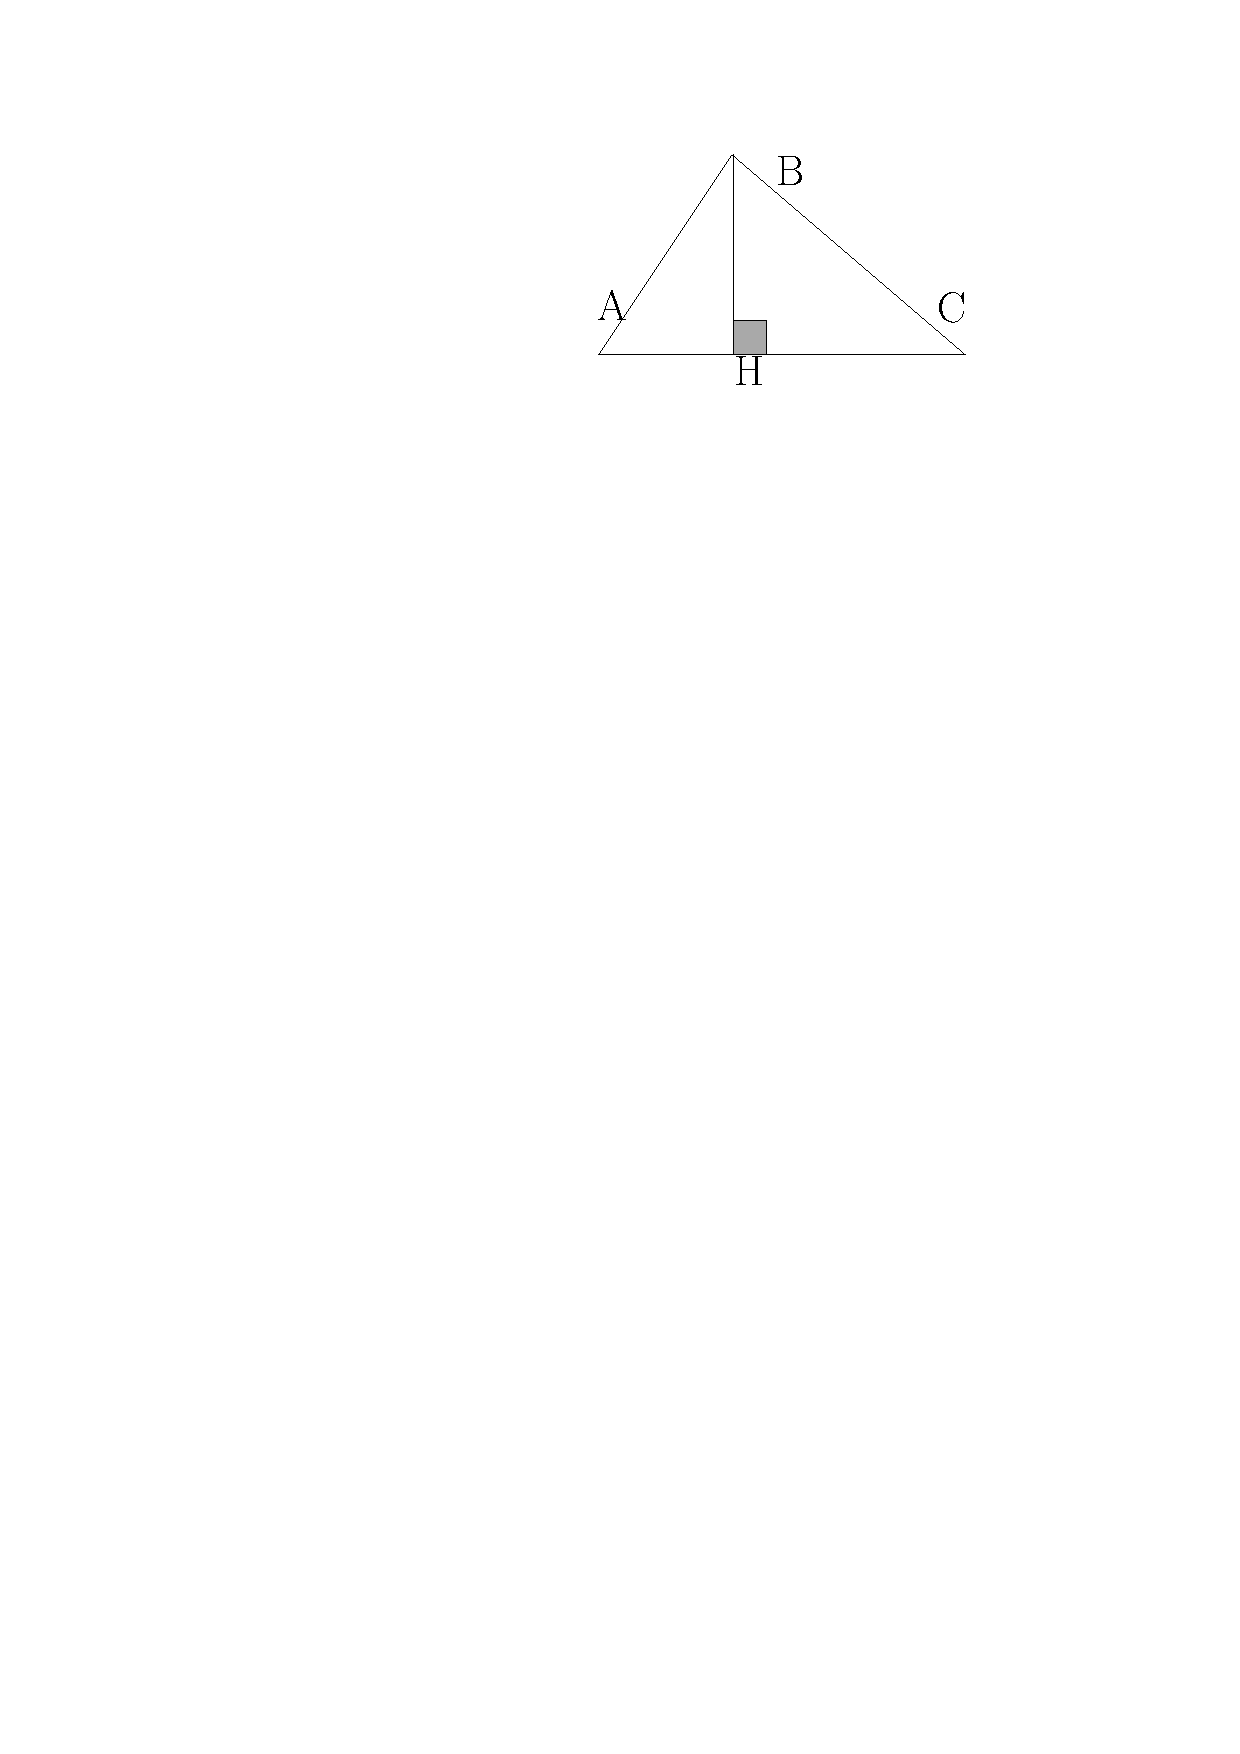
\includegraphics[width=0.9\linewidth]{sources/2/exo4.pdf}
  \end{figure}

  \textit{ \textbf{Calculer tous les angles du triangles ABC}. Justifier.}
  \Pointille[10]
  
  \Pointille[10]
\end{multicols}

Bonus : Quelle est l'utilité du point H ?
\end{document}
